\subsubsection{The LeBlanc Problem}\label{ss:leblanc}

The third shock tube problem is the LeBlanc\footnote{Attempts to find the original citation for this test problem were unsuccessful until William Rider of Sandia NationalLaboratory provided the following information: ``I believe it was called TP37 in the JOWOG 42 structure at the Labs.  The first mention of it in the literature I can find is a AIAA paper by Pember and Anderson (LLNL) \cite{Pember} in 2001.  They also did a longer report comparing methods in 2000 (comparing Eulerian methods to ALE methods with LeBlanc being one of the problems).  They point to a paper by Benson \cite{Benson} as a source along with personal communications with Jim LeBlanc.''} problem.  The setup for this problem is again illustrated in Figure~\ref{fig:shockTube} with initial data  given in Table~\ref{tab:leblancIC}. This is an extreme test problem due to the very small density ratio of $10^{-3}$ and pressure ratio of $10^{-9}$.  The parameter input files for Flexi is in \ref{ssec:flexiin-leblanc} and for hopr \ref{ssec:hoprin-leblanc}. Results are show for $t = 6.$ in Figure~\ref{fig:CVleblanc} for conserved variables while primitive variables are shown in Figure~\ref{fig:PVleblanc}.

\begin{table}[h!]
 \begin{center}
  \caption{Initial conditions for LeBlanc's test case.}
  \label{tab:leblancIC}
  \begin{tabular}{|c|ccc|cccc|cccc|} \hline
   \textbf{Case} & \multicolumn{3}{c|}{\textbf{Domain}} & \multicolumn{4}{c|}{\textbf{Left Gas}} & \multicolumn{4}{c|}{\textbf{Right Gas}} \\ \hline
   \multirow{2}{*}{$1$} & $x_L$ & $x_D$ & $x_R$ & $\rho$ & $u$ & $P$ & $\gamma$ & $\rho$ & $u$ & $P$ & $\gamma$ \\ \cline{2-12}
   \multicolumn{1}{|c|}{} & 0. & 3. & 9.  & 1. & 0. & 2/3 E-1 & 5/3 & 1.E-3 & 0. & 2/3 E-10 & 5/3 \\ \hline
  \end{tabular}
 \end{center}
\end{table}

\begin{figure}[h!]
 \centering
 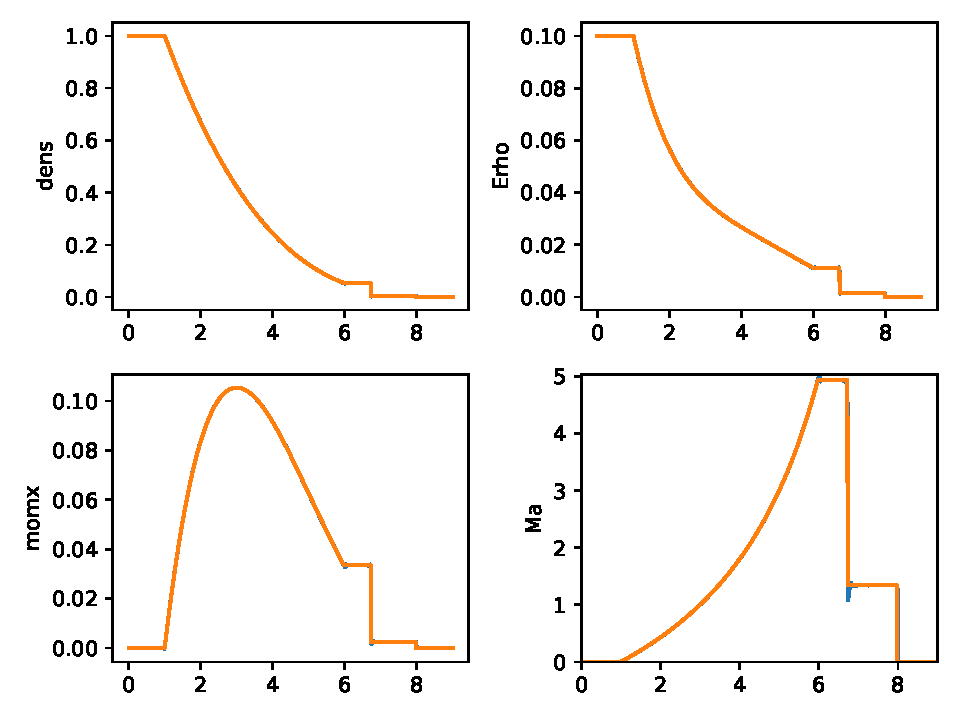
\includegraphics[scale=0.8]{figures/leblanc-CV.pdf}
 \caption{LeBlanc problem at $t = 6.$ with 100 equal sized elements in the $x$-direction showing the conserved variables.  Comparison is made to the exact solution (in red.)  The derived Mach number shows slight variation from the exact solution at the shock front, but the conserved variables are nearly identical to it.}
 \label{fig:CVleblanc}
\end{figure}

\begin{figure}[h!]
 \centering
 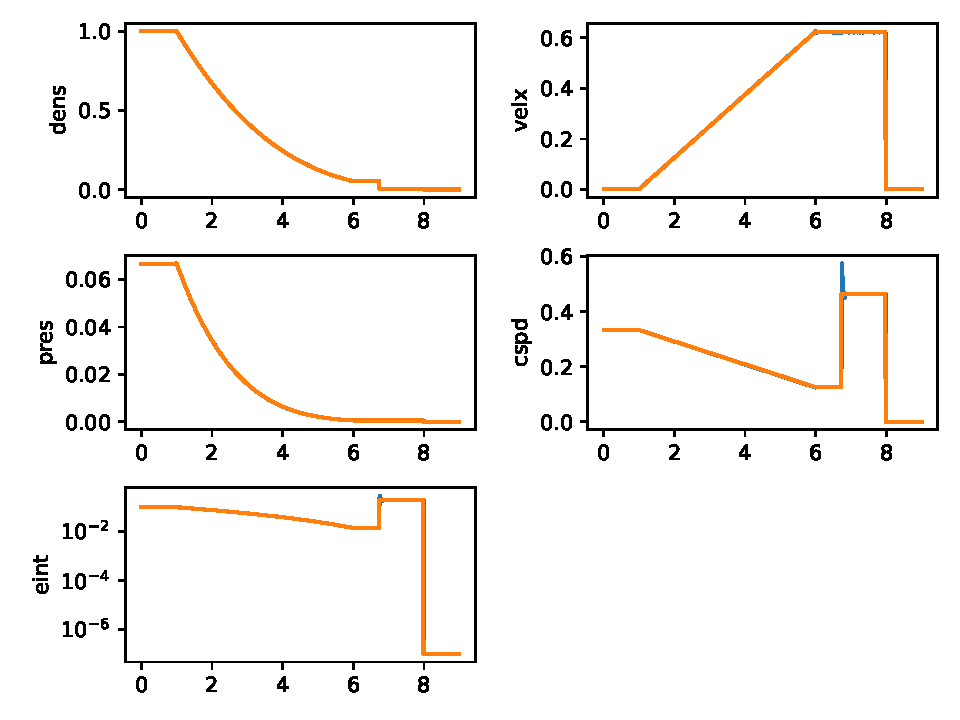
\includegraphics[scale=0.8]{figures/leblanc-PV.pdf}
 \caption{LeBlanc problem at $t = 6.$ with 100 equal sized elements in the $x$-direction showing primitive variables.  Comparison is made to the exact solution (in red.)}
 \label{fig:PVleblanc}
\end{figure}
\noindent Table~\ref{tab:leblancEps} shows the average error in the Flexi solution to be less than $9.04E-4$.

\begin{table}[h!]
 \centering
 \begin{tabular}{|c|c|} \hline
   Variable & $\bar{\epsilon}$ \\ \hline \hline
   $\rho$ & 1.41E-4 \\
   $m_x$  & 1.11E-4 \\
   $E$      & 6.47E-5 \\ \hline
   $v_x$  & 9.04E-4 \\
   $u$     & 5.76E-4 \\
   $P$     & 2.67E-5 \\ \hline
 \end{tabular}
 \caption{Average error (\textit{c.f.,} Eq.~\ref{eq:error}) for the LeBlanc Problem}\label{tab:leblancEps}
\end{table}

\paragraph{Conclusions}

Flexi performs very well on the LeBlanc problem with only minor overshoot at the shock front.
